\documentclass[10pt,two column,letter paper]{article}
\usepackage{cvpr}
\usepackage{times}
\usepackage{epsfig}
\usepackage{graphicx}
\usepackage{amsmath}
\usepackage{amssymb}
\usepackage{cite}

% Include other packages here, before hyperref.

% If you comment hyperref and then uncomment it, you should delete
% egpaper.aux before re-running latex.  (Or just hit 'q' on the first latex
% run, let it finish, and you should be clear).
\usepackage[breaklinks=true,bookmarks=false]{hyperref}

\cvprfinalcopy % *** Uncomment this line for the final submission

\def\cvprPaperID{****} % *** Enter the CVPR Paper ID here
\def\httilde{\mbox{\tt\raisebox{-.5ex}{\symbol{126}}}}

% Pages are numbered in submission mode, and unnumbered in camera-ready
%\ifcvprfinal\pagestyle{empty}\fi
\setcounter{page}{4321}
\begin{document}

%%%%%%%%% TITLE
\title{Laboratory 7 - PHOW Classification}

\author{Ricardo MENDOZA-LEON\\
Universidad de los Andes\\
Bogot\'{a} Colombia\\
{\tt\small ra.mendoza35@uniandes.edu.co}
}

\maketitle
%\thispagestyle{empty}

%%%%%%%%% ABSTRACT
\begin{abstract}
Image content classification in an important task wit several applications in computer vision 
problems. Results of several experiments in multiclass image classification using textons 
to classify textured images are reported. Two different classifiers: nearest-neighborhood (NN) 
and random forest, were trained with k-means quantized histograms of texton responses on 750
train images, and tested in a dataset of 250 images. Results showed better scores for 
random forest classifiers, specially when the number of trees was increased.
However, NN classifier performance was comparable, confirming that a suitable representation
for the problem at hand is key.
\end{abstract}

%%%%%%%%% BODY TEXT
\section{Dataset}
In this lab, two datasets were used. The first one is Caltech101, wich contains 102 classes
totaling 3000 color images, with uneven number in each class. This are images of everyday
scenes, but taken by photograpers. Mayor variability is reflected in inter-class variability, 
beign most of the images in the same class very similar, with orientation normalized using
cropping and rotations.

The second dataset is a subset of imagenet-tiny dataset, wich contains 200 classes totaling 20.000 
color images, from Flickr. Contrary to Caltech101, this dataset has an even number of images
in each class (100 in each class). Variability in this images is high; noteworty is the
intra-class variability (much more than Caltech101). Also the various scales and locations
of classes, the multiplicity of instances that can appear in an image and the background
complexity, make this dataset very complex and challenging.






\section{Methods}
The base recognition pipeline $PHOW_CALTECH101$ implemented by Andrea Vedaldi, is very similar to the one described in the lab6. The mayor stages are:

A) Dictionary creation: After image setup, this method, instead of using a bank of filters, the base descriptor is the Pyramid Histogram of Oriented Gradients (PHOG), that
calculates histograms of gradient orientations for a number of regions inside a window centered at regular steps in the image. Given that is a multiscale model
(pyramid), this process divides the window along the $x$ and $y$ axis (spatial divisions $sDivX$, $sDivY$) at different heights or $levels$; the number
of orientation bis are usually 8. With this procedure, a feature vector is extracted at each window location. Then, features are quantized to a number
of given words $k$. In Andrea's pipeline, quantization is obtained by using k-means, then creates a space division tree (KD-Tree) as a lookup structure which
 offers a very fast way to label new vectors (by traversing the tree ideally in log(k) steps).

B) Classifier training and prediction: A set of binary classifiers is trained to recognize examples of each class. The classifiers used are SVMs with a  
Stochastic Dual Coordinate Ascent SDCA kernel. Later, in the prediction step given a image representation, the class corresponding to the maximum confidence
value for all classifiers is used to label the image. For tests in imagenet-tiny we used 90\% of images for training and 10\% for test.


\section{Results and discussion}
Figure ~\ref{fig:bar_all} summarizes the global performance for different experiments. A first test was run using the caltech101 dataset with an equal
number of images for training and test, using the default settings of Andrea's code ($k=$600 and two level PHOG with $sDivX=sDivY=[2,4]$) for 102 classes.
The score matrix for train and test images, and the confusion matrix for the classification task are shown in figures ~\ref{fig:calt_A} and ~\ref{fig:calt_B}, 
were it can be observed a global accuracy of 68.10\%. However, it can be noticed in the confusion matrix some classes whose accuracy is very low 
(dark blue values at the diagonal), but its correspondig value in the train scores matrix is high, meaning over-fitting ocurred
for that class classifier. Noteworty are the first five classes in the dataset that have allmost 100\% accuracy.

Different configurations of dictionary and spatial partitioning were tested on imagenet-tiny dataset. Figure ~\ref{fig:m1_imagenet_tiny} and ~\ref{fig:m1-2_imagenet_tiny},
shows the results for imagenet-tiny dataset with parameters $k=$600 and two level PHOG with $sDivX=sDivY=[2,4]$ in 200 classes. The first thing to notice is the low
accuracy obtained for this dataset, which is caused by the much higher variability, but also the hiegher granularity of the classes. For instance, the 
chihuahua class had 0\% accuracy as shown in figure ~\ref{fig:m1_imagenet_tiny_chihuahua_1}. Furthermore, confusion and score matrices 
(figure ~\ref{fig:m1_imagenet_tiny_chihuahua_2}) reveal missclassification with the class English\_springer (figure ~\ref{fig:English_springer}), which is
and cathegorically close to Chihuahua (figure ~\ref{fig:chihuahua}). 

An additional set of parameters $k=$1200 and $sDivX=sDivY=[2, 4]$ in 200 classes, and $k=$600 with $sDivX=sDivY=[4, 8]$ in 50 classes, 
was tested on the imagenet-tiny (figures ~\ref{fig:m2_imagenet_tiny} and ~\ref{fig:m2-2_imagenet_tiny}, and ~\ref{fig:m14_imagenet_tiny} and ~\ref{fig:m14-2_imagenet_tiny}),
which improved the accuracy to 28.65\% and 37.40\% respectibly. An analysis for the Chihuahua class, showed no improvement for this class as seen the confusion and score matrices 
(figures ~\ref{fig:m2_imagenet_tiny_chihuahua_1} and ~\ref{fig:m2_imagenet_tiny_chihuahua_2}, and ~\ref{fig:m14_imagenet_tiny_chihuahua_1} and ~\ref{fig:m14_imagenet_tiny_chihuahua_2}).
However we note the inclussion of the EntleBucher class ~\ref{fig:EntleBucher}. In conclussion the PHOG descriptor was uncapable of representing the distintive features for class Chihuahua.
Similar results occur with other classes in this dataset, hindering improvements.



\begin{figure}[t]
\begin{center}
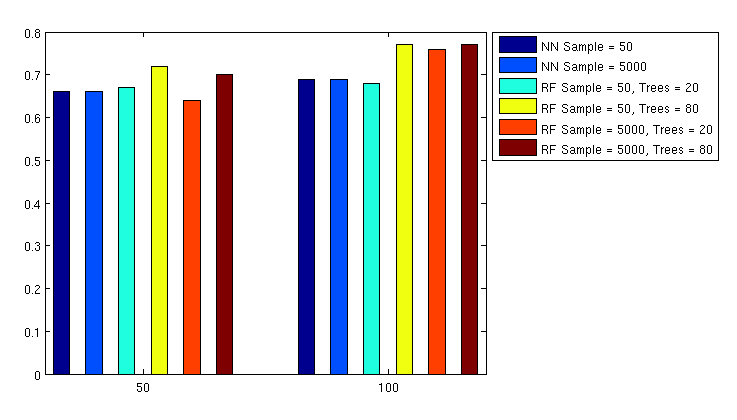
\includegraphics[width=0.9\linewidth]{bar_all.png}
\end{center}
   \caption{summary results for all tests}
\label{fig:bar_all}
\end{figure}

\begin{figure*}[t]
\begin{center}
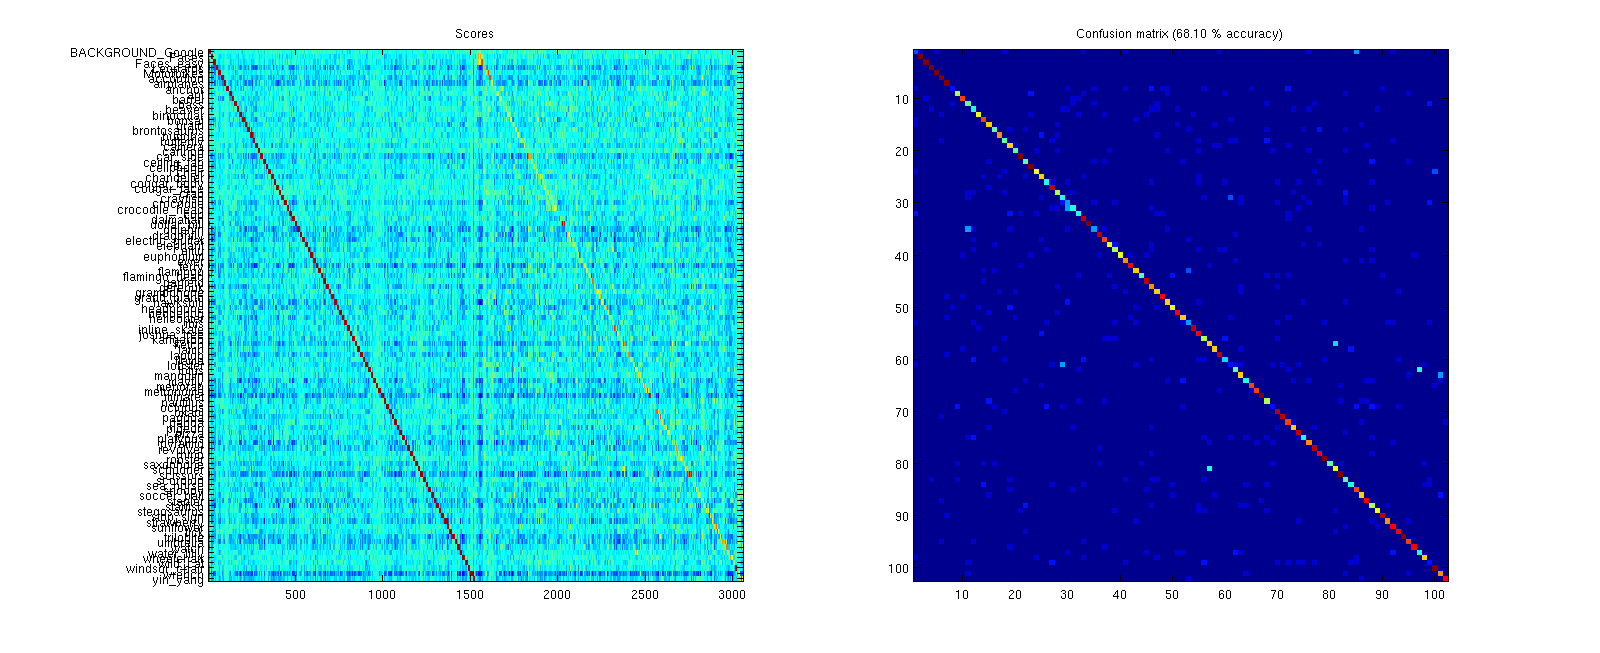
\includegraphics[width=0.9\linewidth]{caltech101_baseline.png}
\end{center}
   \caption{}
\label{fig:calt_A}
\end{figure*}

\begin{figure*}[t]
\begin{center}
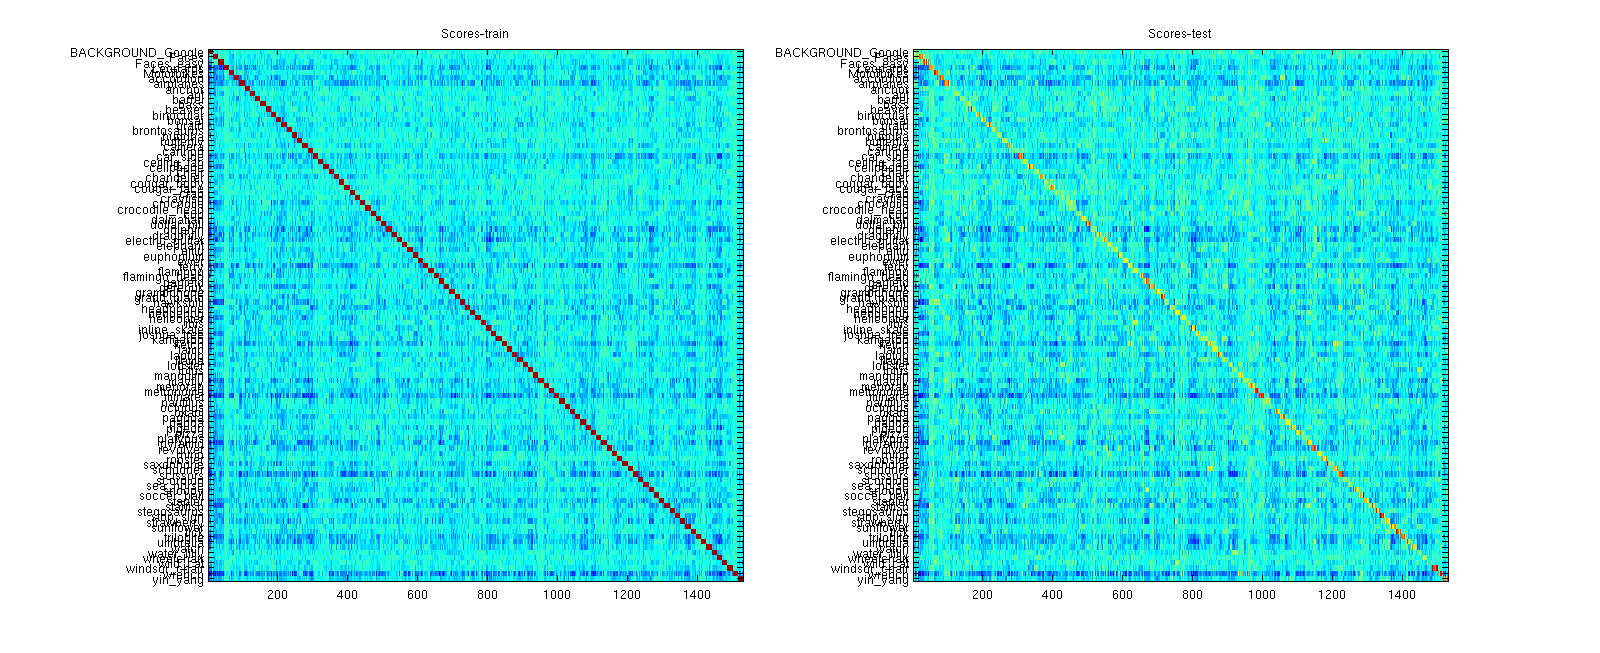
\includegraphics[width=0.9\linewidth]{caltech101-2_baseline.png}
\end{center}
   \caption{}
\label{fig:calt_B}
\end{figure*}

\begin{figure*}[t]
\begin{center}
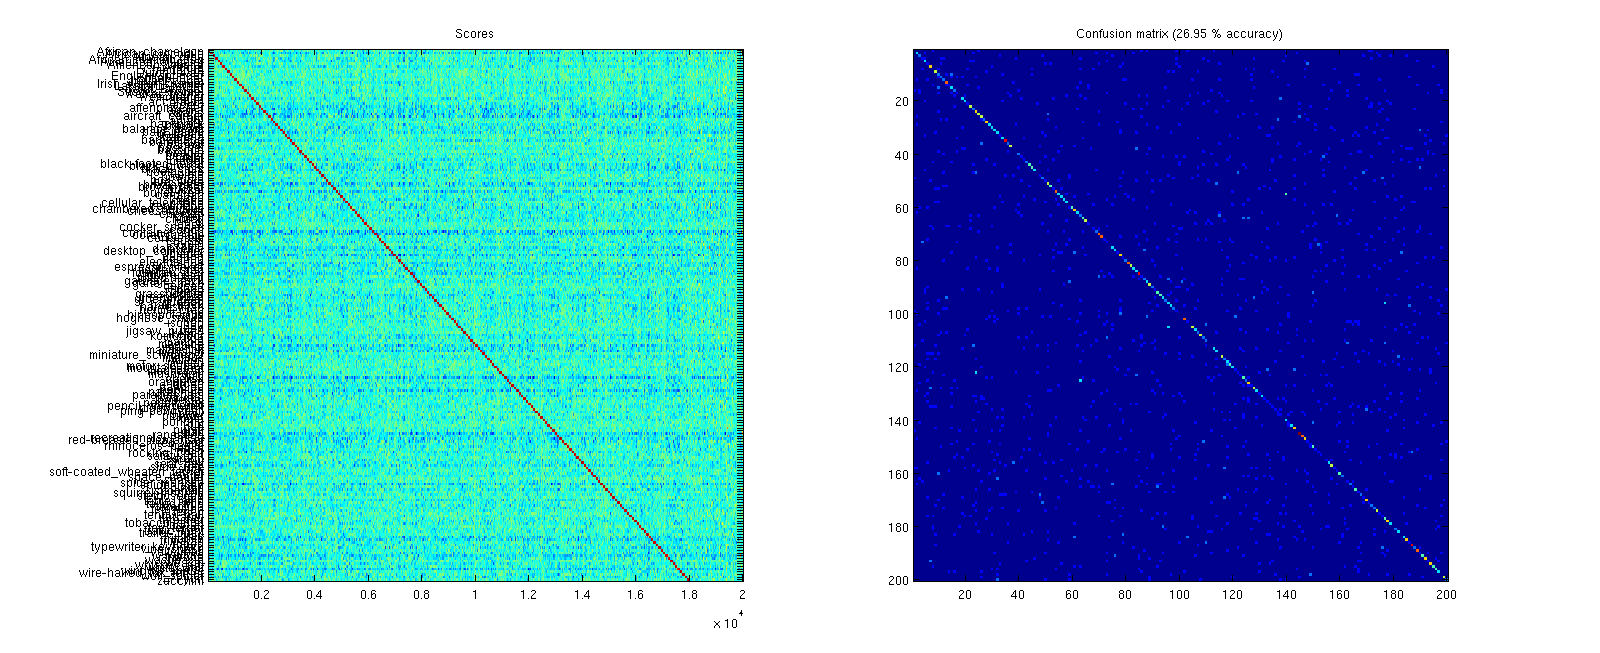
\includegraphics[width=0.9\linewidth]{m1_imagenet_tiny.png}
\end{center}
   \caption{}
\label{fig:m1_imagenet_tiny}
\end{figure*}

\begin{figure*}[t]
\begin{center}
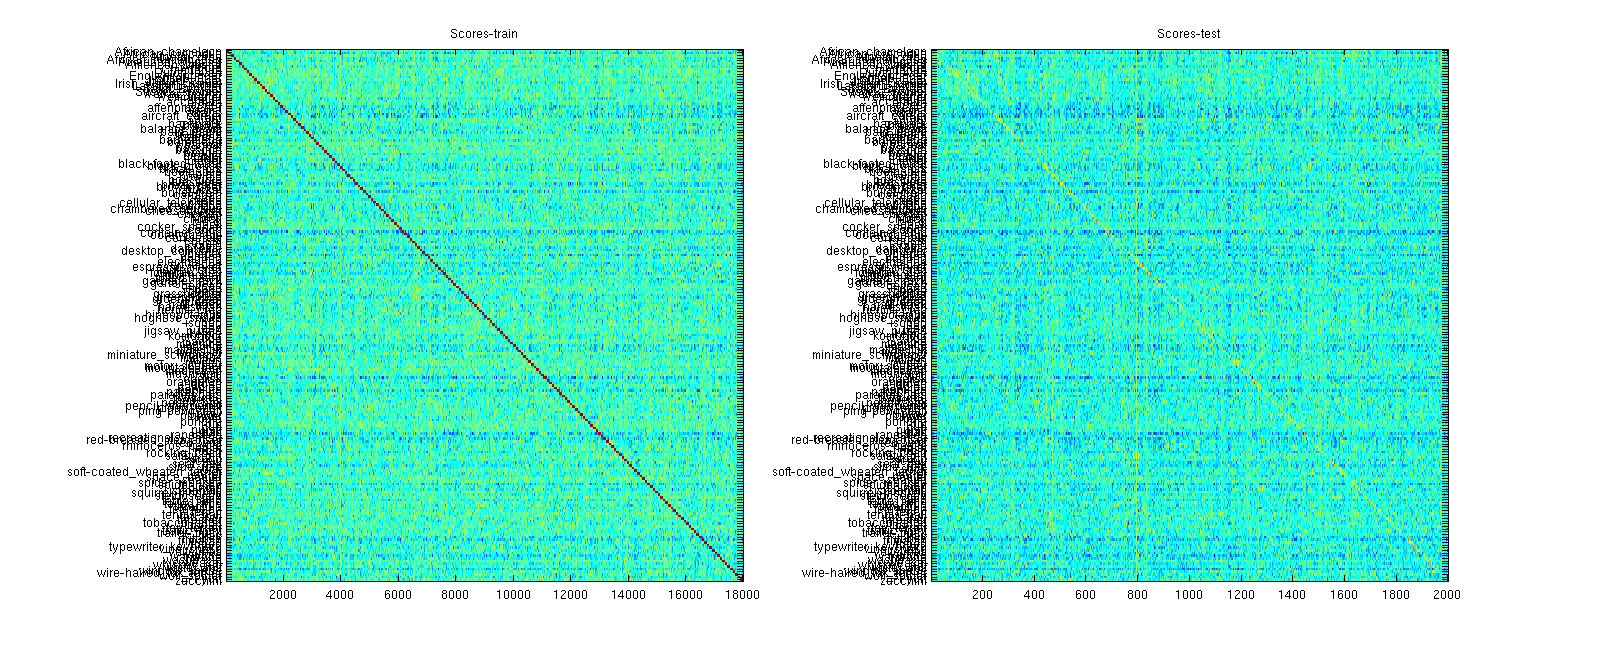
\includegraphics[width=0.9\linewidth]{m1-2_imagenet_tiny.png}
\end{center}
   \caption{}
\label{fig:m1-2_imagenet_tiny}
\end{figure*}

\begin{figure}[t]
\begin{center}
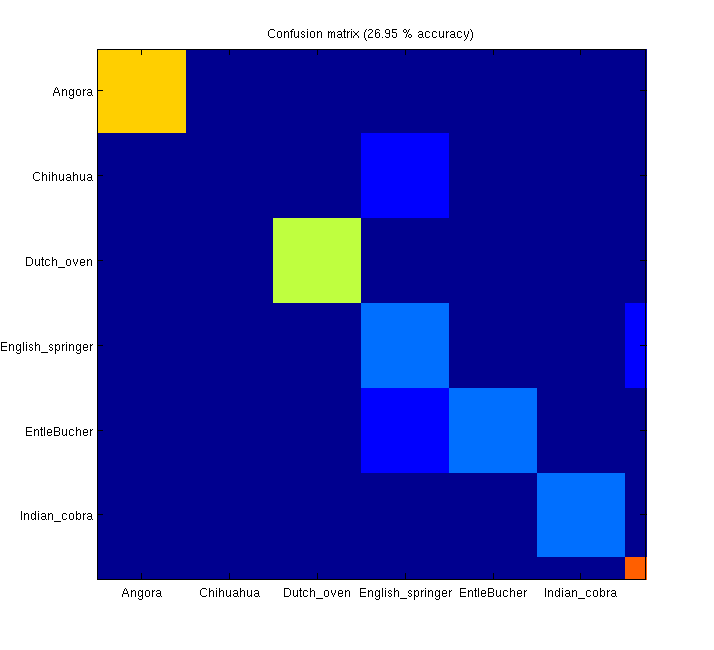
\includegraphics[width=0.9\linewidth]{m1_imagenet_tiny_chihuahua-1.png}
\end{center}
   \caption{}
\label{fig:m1_imagenet_tiny_chihuahua_1}
\end{figure}

\begin{figure}[t]
\begin{center}
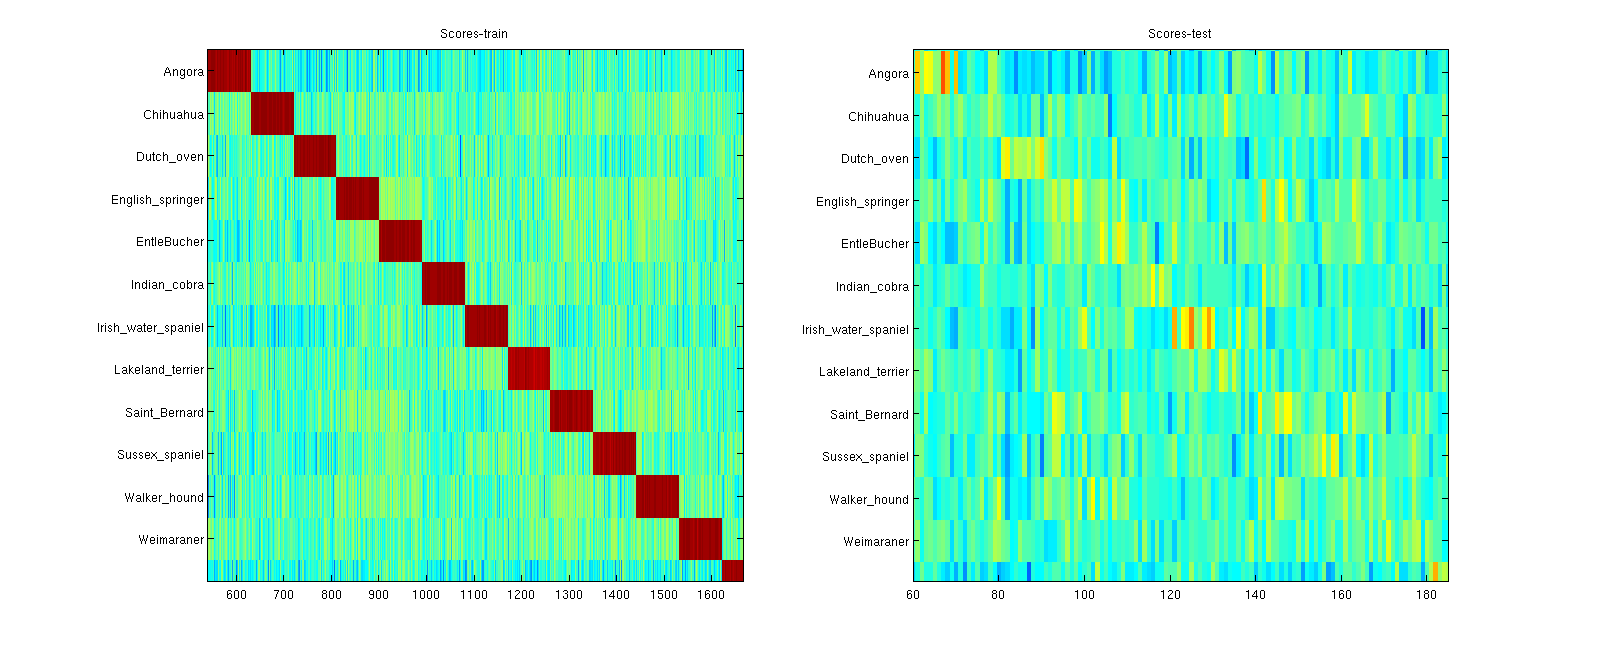
\includegraphics[width=0.9\linewidth]{m1_imagenet_tiny_chihuahua-2.png}
\end{center}
   \caption{}
\label{fig:m1_imagenet_tiny_chihuahua_2}
\end{figure}

\begin{figure}[t]
\begin{center}
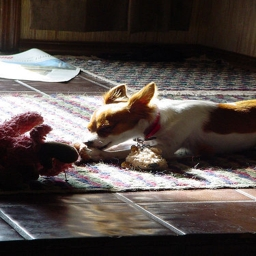
\includegraphics[width=0.9\linewidth]{chihuahua.JPEG}
\end{center}
   \caption{}
\label{fig:chihuahua}
\end{figure}

\begin{figure}[t]
\begin{center}
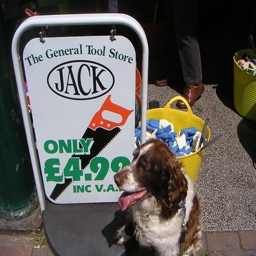
\includegraphics[width=0.9\linewidth]{English_springer.JPEG}
\end{center}
   \caption{}
\label{fig:English_springer}
\end{figure}

\begin{figure}[t]
\begin{center}
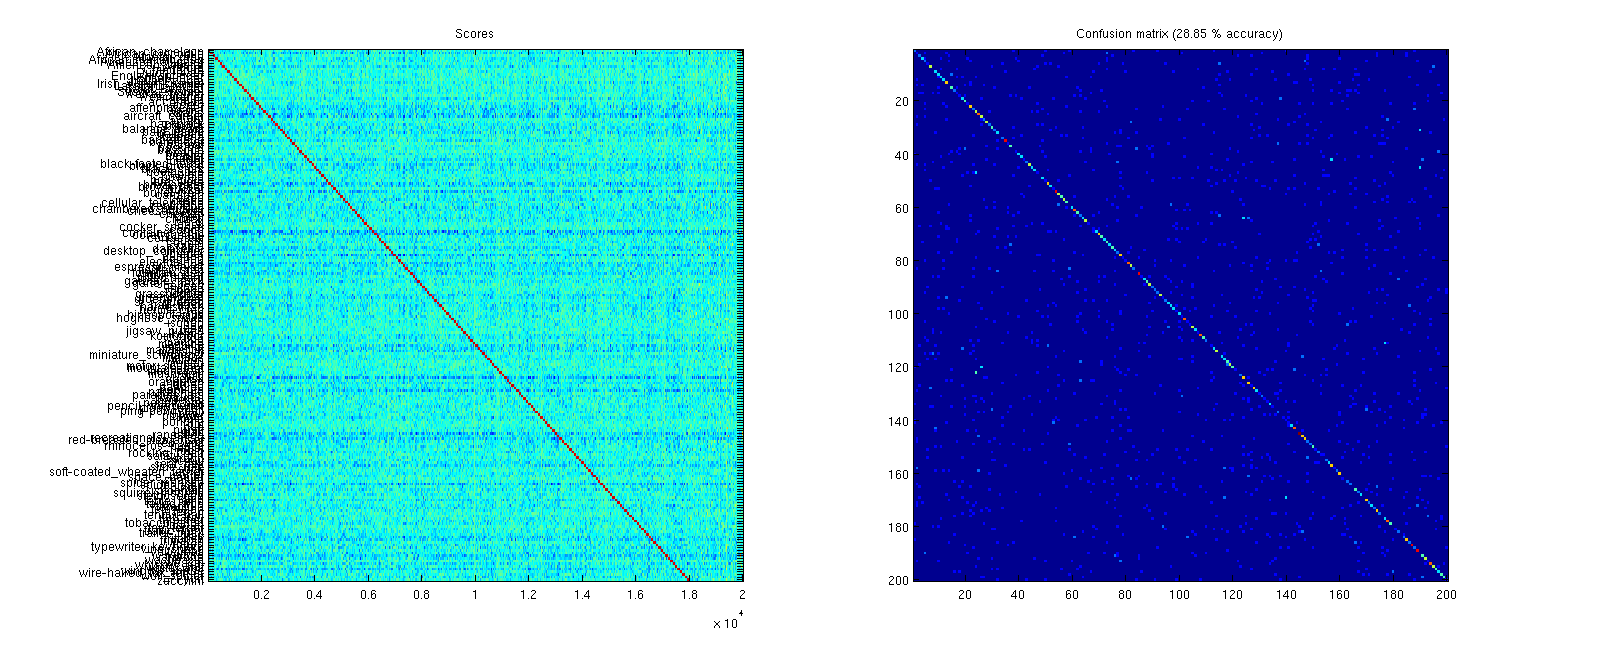
\includegraphics[width=0.9\linewidth]{m2_imagenet_tiny.png}
\end{center}
   \caption{}
\label{fig:m2_imagenet_tiny}
\end{figure}

\begin{figure}[t]
\begin{center}
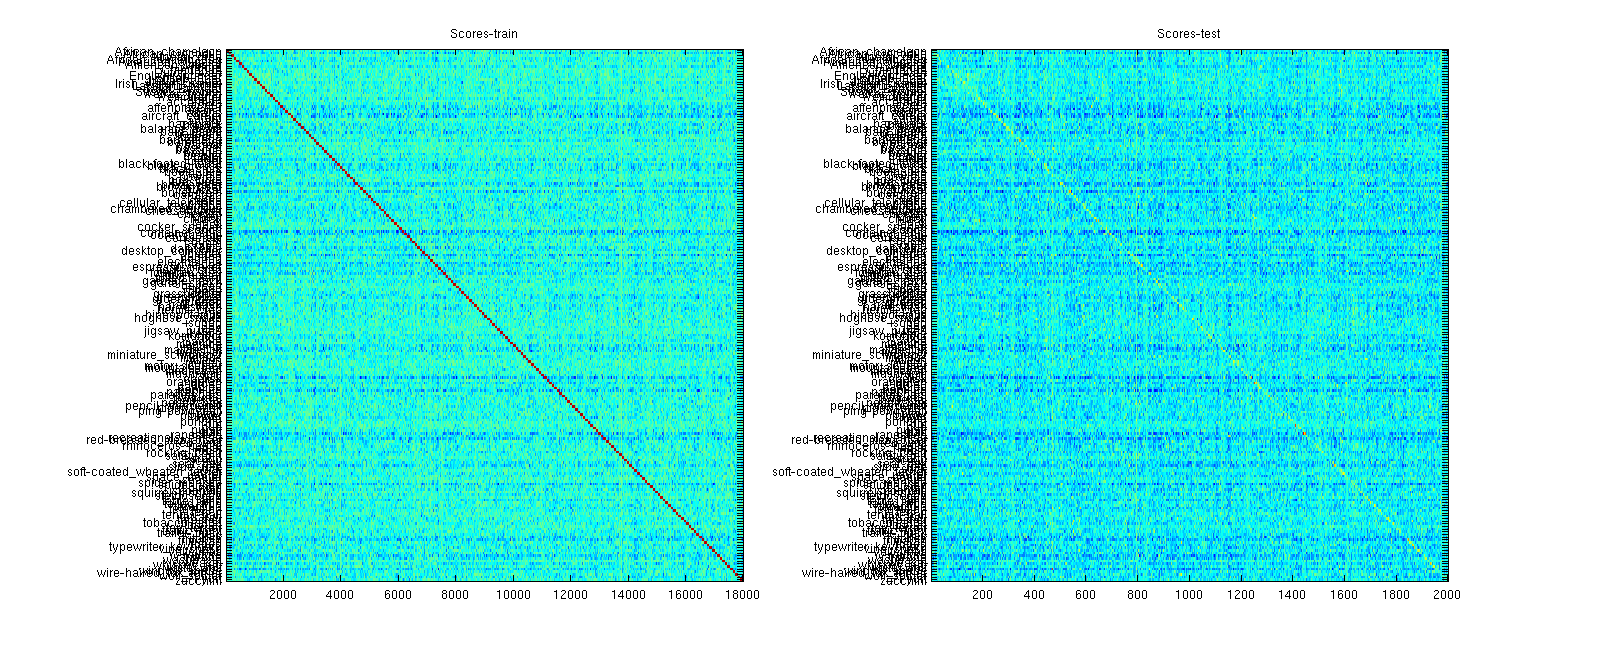
\includegraphics[width=0.9\linewidth]{m2-2_imagenet_tiny.png}
\end{center}
   \caption{}
\label{fig:m2-2_imagenet_tiny}
\end{figure}

\begin{figure}[t]
\begin{center}
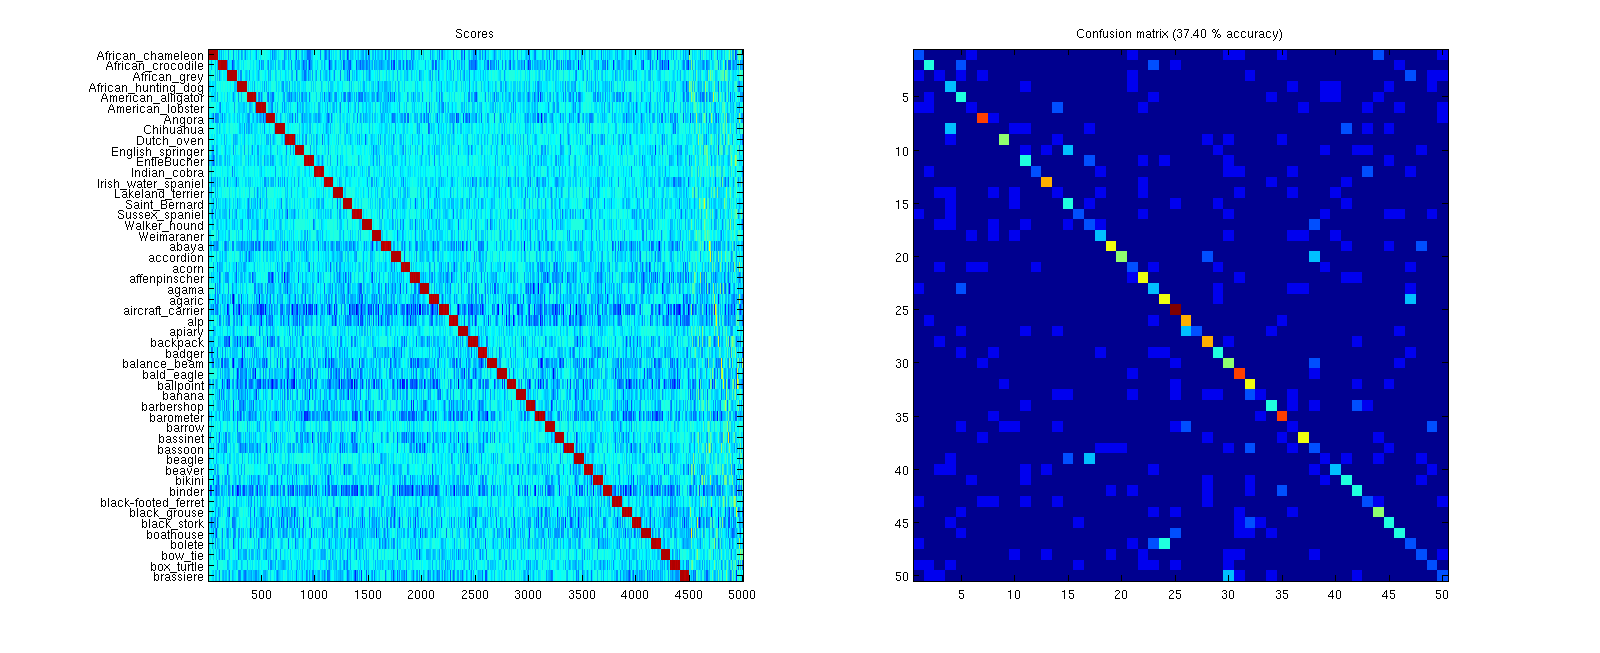
\includegraphics[width=0.9\linewidth]{m14_imagenet_tiny.png}
\end{center}
   \caption{}
\label{fig:m14_imagenet_tiny}
\end{figure}

\begin{figure}[t]
\begin{center}
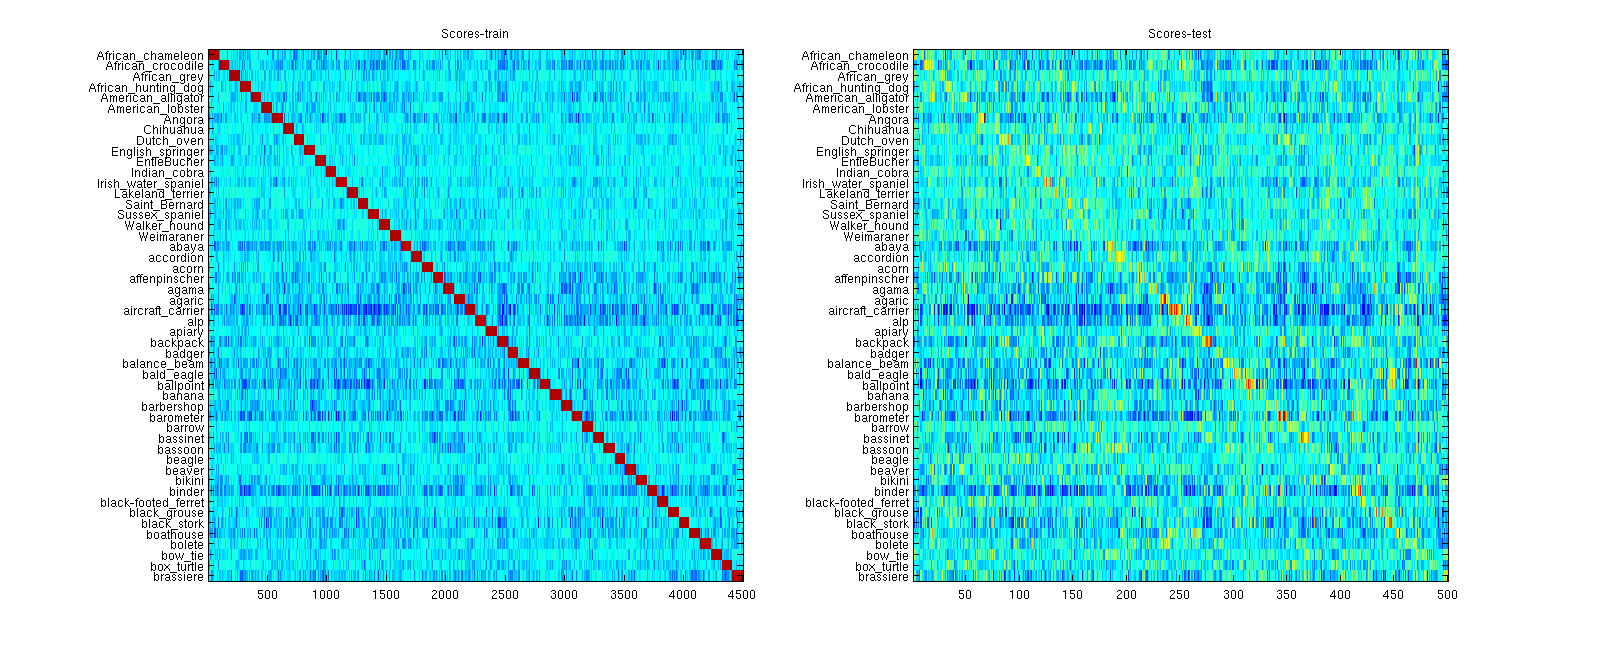
\includegraphics[width=0.9\linewidth]{m14-2_imagenet_tiny.png}
\end{center}
   \caption{}
\label{fig:m14-2_imagenet_tiny}
\end{figure}

\begin{figure}[t]
\begin{center}
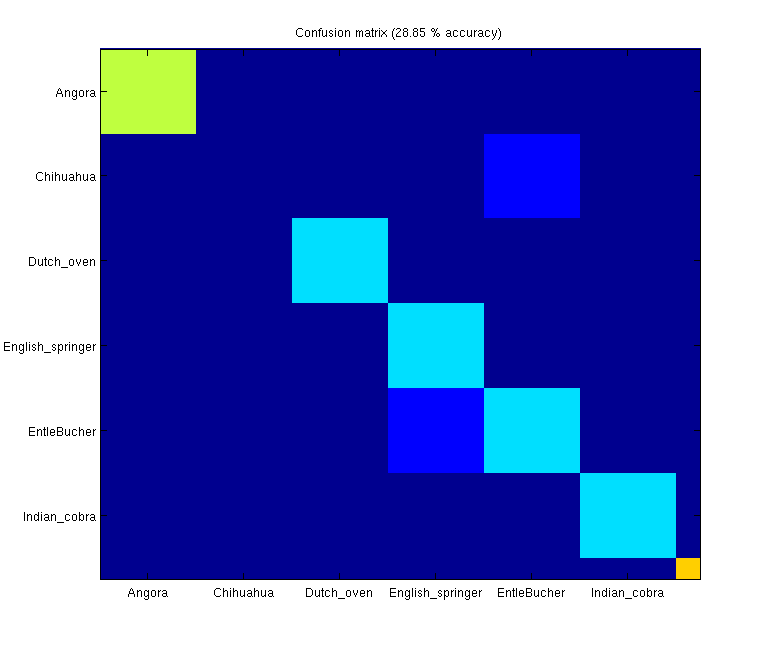
\includegraphics[width=0.9\linewidth]{m2_imagenet_tiny_chihuahua-1.png}
\end{center}
   \caption{}
\label{fig:m2_imagenet_tiny_chihuahua_1}
\end{figure}

\begin{figure}[t]
\begin{center}
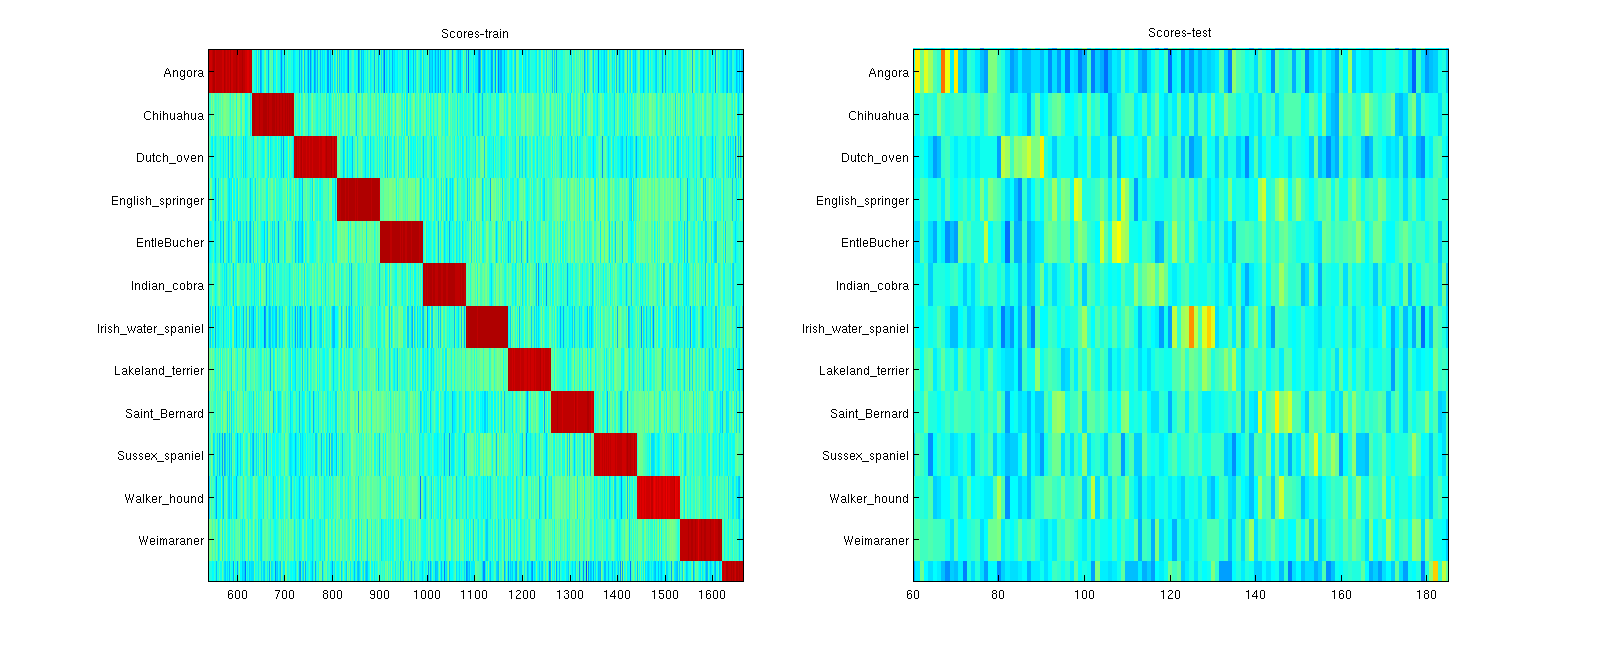
\includegraphics[width=0.9\linewidth]{m2_imagenet_tiny_chihuahua-2.png}
\end{center}
   \caption{}
\label{fig:m2_imagenet_tiny_chihuahua_2}
\end{figure}


\begin{figure}[t]
\begin{center}
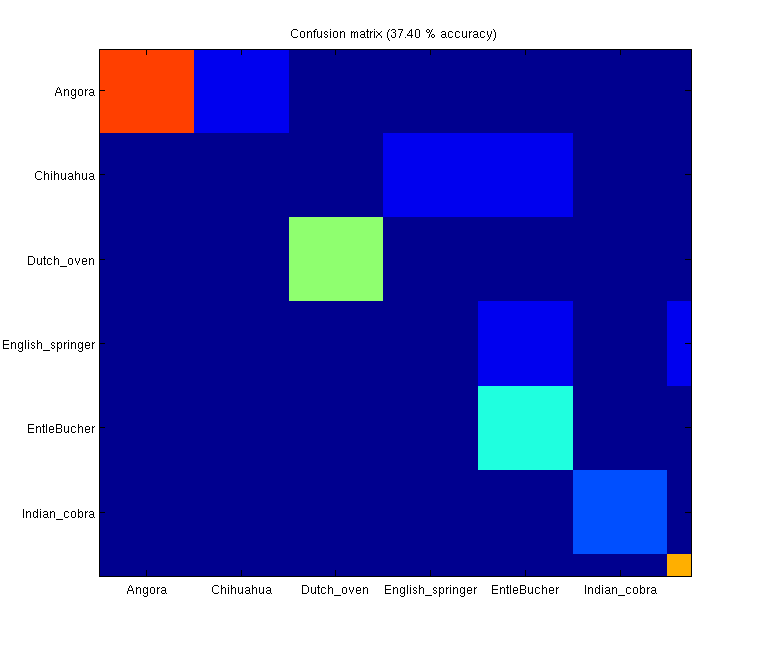
\includegraphics[width=0.9\linewidth]{m14_imagenet_tiny_chihuahua-1.png}
\end{center}
   \caption{}
\label{fig:m14_imagenet_tiny_chihuahua_1}
\end